\section{Proces}
De ontwerp en realisatie fases van het project worden ondersteund door middel van de scrum methodiek \Parencite{Scrum}.
Tijdens de realisatieperiode worden alle fases van de \gls{SDLC} (figuur \ref{fig:SLDC}) doorlopen.\\
% Hierbij wordt de requirement analysis uitgevoerd aan de hand van het onderzoek. gcc
% Daarna worden er 2 weken geplant voor het designen van het systeem.
% Vervolgens worden er 9 sprints geplant voor het implementeren en testen van het systeem. \\
\begin{graphic}
	\vspace{0.2cm}
	\captionsetup{type=figure}
	\caption{De Software Development Life Cycle, afkomstig uit de afstudeerhandleiding \Parencite{Afstudeerhandleiding}} % \Parencite{Afstudeerhandleiding}
	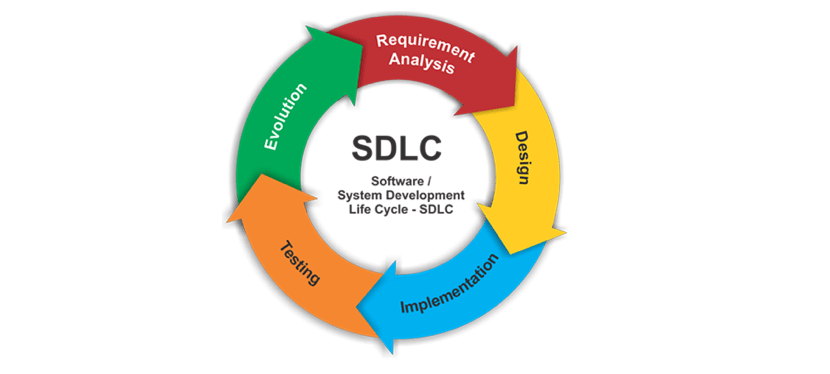
\includegraphics[scale=0.4]{SDLC}
	\label{fig:SLDC}
	\vspace{0.2cm}
\end{graphic}
% \todo[inline]{Bron van afstudeerhandleiding fixen}
\textbf{Requirement analysis:} Door middel van de requirement analyse (het onderzoek dat beschreven staat in hoofdstuk \ref{chap:Onderzoek}) worden de requirements opgesteld.
Tijdens de sprint planning worden de requirements verwerkt tot behapbare user stories, zodat ze tijdens de sprints gemaakt kunnen worden.\\
\textbf{Design:} De eisen en wensen die vanuit de requirement analyse worden gehaald worden gebruikt om een ontwerp te maken.
Hoe er ontworpen wordt is toegelicht in hoofdstuk \ref{sec:Ontwerpen}.\\
%
% De eisen en wensen die vanuit de requirement analyse worden gebruikt om het ontwerp te maken.
% Hoe er ontwerpt wordt is toegelicht in hoofdstuk \ref{sec:Ontwerpen}.\\
\textbf{Inplementation:} De eisen en wensen worden geïmplementeerd volgens het ontwerp.\\
\textbf{Testing:} Door de loop van het realisatieproces worden de verschillende testen van het V-Model uitgevoerd, zie hoofdstuk \ref{sec:Testing} voor meer informatie.\\
\textbf{Evolution:} Er wordt met regelmaat feedback momenten gehouden waar het product gedemonstreerd wordt aan de bedrijfsbegeleider.
Dit wordt gedaan om de projectvoortgang te bewaken op basis van de gemaakte eisen en wensen.
\subsection{Code reviews}
Tijdens de realisatiefase worden er meerdere code reviews gehouden om de codekwaliteit te waarborgen.
Deze code reviews worden gehouden met de backend en frontend developers van Snakeware, de code zal beoordeeld worden op coderingsstandaarden en structuur.
\subsection{Versiebeheer}
Binnen Snakeware wordt er gebruikgemaakt van Bitbucket \Parencite{BitBucket} en git \Parencite{Git} voor het versiebeheer van de code, dit zal ook gebruikt worden voor de afstudeeropdracht.
Verder zal er ook gebruikgemaakt worden van een CI-pipeline die wordt opgezet om de code automatisch te testen.
